\documentclass[letterpaper]{article}

\usepackage[submission]{aaai2027}
\usepackage[hyphens]{url}
\usepackage{graphicx}
\urlstyle{rm}
\def\UrlFont{\rm}
\usepackage{natbib}
\usepackage{caption}
\frenchspacing
\usepackage{amsmath}
\usepackage{amssymb}
\usepackage{booktabs}
\usepackage{array}

\pdfinfo{
/TemplateVersion (2027.1)
}

\graphicspath{{figures/}}

\newcommand{\method}{CanonDressGS}
\newcommand{\dual}{Dual-Support}
\newcommand{\pending}{\textemdash}
\newcommand{\figureplaceholder}[3]{%
    \fbox{%
        \parbox[c][#1][c]{0.96\linewidth}{%
            \centering
            \textbf{#2}\\[1.5mm]
            \small #3
        }%
    }%
}

\title{\method: Geometry-Safe Reference-Controlled Garment Editing in Canonical Gaussian Space}

\author{Anonymous Submission}
\affiliations{}

\begin{document}

\maketitle

\begin{abstract}
Animatable Gaussian avatars are typically tied to the garments observed during reconstruction, which limits their reuse as editable digital humans.
We present \method{}, a reference-controlled garment editing framework that modifies a frozen animatable Gaussian avatar in canonical space.
Our central observation is that directly interpolating garment-dependent Gaussian geometry produces invalid intermediate supports: Gaussian centers, scales, and rotations move through unsupported configurations, leading to cloud-like artifacts, boundary scatter, and silhouette discontinuities.
To avoid this failure, we first optimize a valid canonical \emph{Teacher Endpoint} for every garment in a closed wardrobe, organize the endpoints in an explicit coordinate system, and map one or more garment reference images to this space with a lightweight set-based predictor.
The automatic single-garment path then snaps the raw prediction to the nearest valid endpoint, guaranteeing that the realized avatar uses an optimized garment state rather than an unconstrained intermediate field.
This representation is more expressive than a bare hard-lookup interface because it exposes coefficient-valued garment states and supports geometry-aware composition, while the deployed endpoint path deliberately retains snapping for robustness.
On THuman4.0 subject02 with five seen garments, \method{} selects all 60 clean queries correctly over 12 cross-fit controller runs, with exact endpoint realization, zero observed identity contamination, and no severe wrong-outfit failures.
The unsnapped predictor already locates the correct endpoint region with 1.0 top-1 accuracy, but obtains zero exact endpoint matches and an endpoint-render LPIPS of 0.0679; snapping raises exact match to 1.0 and reduces the parity LPIPS to $3.19\times10^{-7}$, while clean classifier and nearest-centroid lookup are functionally equivalent when they select the same endpoint.
For mixed garment states, an oracle/user-specified \dual{} extension preserves two valid endpoint geometries and improves LPIPS from 0.0853 to 0.0570, silhouette IoU from 0.7101 to 0.7253, and boundary F-score from 0.3003 to 0.3791 over direct geometry interpolation across all ten garment pairs.
A second-identity replication on subject00 is included in the evaluation protocol; its quantitative entries are intentionally left blank in this draft pending sealed results.
\end{abstract}

% --------------------------------------------------------------------------
% Figure 1: Teaser / task definition. Replace only with real project assets.
% Expected file: figures/figure1_canondressgs_teaser.pdf
% --------------------------------------------------------------------------
\begin{figure*}[t]
    \centering
    \IfFileExists{figures/figure1_canondressgs_teaser.pdf}{
        
\includegraphics[width=\textwidth]{figures/figure1_canondressgs_teaser.pdf}
    }{
        \figureplaceholder{0.19\textheight}
        {Figure 1 Placeholder: Task and Main Results}
        {Garment references $+$ target pose/camera $\rightarrow$ the same animatable identity wearing a selected garment endpoint.\\
        Suggested layout: five subject02 garments; reference inputs; Base Avatar; \method{} result; Teacher Endpoint; representative target poses/cameras.\\
        Add subject00 only after its sealed second-identity results are available.}
    }
    \caption{
    \textbf{Reference-controlled garment editing in canonical Gaussian space.}
    Given one or more garment reference images and a target pose and camera,
    \method{} realizes a valid garment endpoint on a frozen animatable avatar while
    preserving the identity and animation interface. All panels in the final figure
    must come from sealed project outputs.
    }
    \label{fig:teaser}
\end{figure*}

\section{Introduction}

Animatable 3D Gaussian avatars provide efficient free-viewpoint rendering and pose-driven animation, but their reconstructed representation usually entangles identity, body geometry, and the clothing observed during capture.
Replacing the captured garment is therefore not a simple texture-editing problem.
A successful system must coordinate changes in Gaussian position, scale, rotation, opacity, and appearance while preserving the subject identity and remaining compatible with the frozen deformation and rendering backbone.

A direct reference-to-residual predictor appears attractive because it could, in principle, generate arbitrary garment-dependent Gaussian fields.
In practice, however, this mapping is difficult: a small set of garment images must determine a highly localized, high-dimensional residual over roughly two hundred thousand irregularly distributed Gaussians.
Our exploratory diagnostics show that direct dense residual prediction and weak reference-conditioning designs do not reliably recover stable garment structure; the matched evaluation below therefore isolates coefficient prediction, endpoint projection, and hard-lookup controls under one current protocol.
The same frozen avatar can nevertheless represent the target garments when the canonical residual is optimized directly.
This reveals a representation--conditioning mismatch: the avatar support is expressive enough for the seen garment endpoints, while unconstrained reference-conditioned generation is not reliably organized.

A second challenge concerns intermediate garment states.
A hard lookup system can retrieve a stored endpoint, but it offers only discrete switching.
A coefficient-space representation is potentially more expressive because it exposes continuous garment coordinates and can support weighted composition.
Yet naively interpolating Gaussian geometry between two valid endpoints is unsafe.
Our endpoint-anchored causal intervention separates geometry, visibility, and appearance and shows that geometry accounts for nearly the full measured artifact effect.
Geometry is sufficient and necessary for the observed failure in all ten unordered garment pairs.
This result changes the design objective: rather than learning a more aggressive geometry interpolator, the method should preserve valid endpoint supports.

Based on these observations, we propose \method{}.
Offline, we optimize one canonical Teacher Endpoint for each garment on a frozen animatable avatar and organize the resulting residuals in an explicit endpoint coordinate system.
At inference time, clothing-masked reference images are encoded by a frozen feature backbone, aggregated by deterministic mean/max pooling, and mapped to endpoint-space coefficients by a lightweight predictor.
For robust single-garment editing, the raw coefficient is snapped to the nearest valid Teacher Endpoint before frozen deformation and rendering.
For user-specified or oracle mixed states, \dual{} retains both endpoint geometries and combines only their effective contribution, avoiding direct interpolation of Gaussian centers, scales, and rotations.

Hard lookup is a strong baseline in a small closed wardrobe, and clean endpoint classification is saturated in our current benchmark.
Our contribution is therefore not limited to improving five-way classification accuracy.
Instead, \method{} provides a unified canonical representation for: (i) constructing valid garment states on a frozen avatar, (ii) mapping references into an explicit garment coordinate system, (iii) guaranteeing valid-state realization through endpoint snapping, and (iv) enabling geometry-safe composition through \dual{}.
In the matched cross-fit evaluation, the raw coefficient predictor locates the correct endpoint region for every clean query but never reconstructs an endpoint exactly; nearest-valid-state projection closes this realization gap while matching privileged or retrieval-based endpoint selection on the saturated clean task.

Our contributions are:
\begin{itemize}
    \item We introduce a canonical garment editing formulation for a frozen animatable Gaussian avatar, where multi-view optimization produces valid garment-specific Teacher Endpoints over geometry, visibility, and appearance.
    \item We identify Gaussian geometry interpolation as the dominant source of invalid intermediate garment states and derive geometry-safe endpoint realization and \dual{} composition from this causal diagnosis.
    \item We develop a lightweight reference-conditioned endpoint-space predictor with nearest-valid-endpoint snapping, achieving oracle-level clean endpoint realization without garment identity, together with zero identity contamination and safe missing-reference fallback.
    \item We provide a controlled evaluation against unsnapped coefficient regression, classifier lookup, nearest-centroid lookup, hard geometry, and linear geometry interpolation, together with explicit perturbation and representation-scope analyses; a reserved subject00 protocol will test second-identity replication.
\end{itemize}

\section{Related Work}

\paragraph{Animatable human avatars.}
Neural and Gaussian avatar methods reconstruct a person from multi-view or monocular observations and synthesize the subject under target views and poses.
Recent Gaussian representations provide explicit primitives, fast rasterization, and canonical-to-posed deformation.
Most systems, however, reconstruct the person together with the clothing present during capture.
\method{} uses an already trained animatable Gaussian avatar as a frozen backbone and studies post-hoc garment editing in canonical space.

\paragraph{Garment editing and human redressing.}
Image-space virtual try-on methods synthesize a dressed person in a single image, while explicit 3D garment-transfer approaches often require garment meshes, templates, simulation, or per-garment reconstruction.
Our setting is complementary: the target is an existing animatable identity whose deformation and renderer should remain unchanged.
The input is one or more garment references, and the output is a reusable canonical garment state that can be animated by the original avatar backbone.

\paragraph{Structured Gaussian control.}
Structured Gaussian methods use anchors, feature grids, local networks, blendshape-like bases, or compact latent codes to control large sets of Gaussian attributes.
These methods motivate separating a high-dimensional spatial representation from a low-dimensional controller.
\method{} differs in the failure being addressed.
Each optimized garment endpoint is individually valid, yet direct interpolation between endpoint geometries can be invalid.
We therefore organize optimized states explicitly and restrict automatic realization to valid endpoints, while retaining a geometry-safe composition operator for controlled intermediate states.

% Keep all currently screened bibliography entries visible until Related Work is expanded.
\nocite{*}

\section{Method}

\subsection{Overview}

The method contains four stages: offline Teacher Endpoint construction, an explicit endpoint coordinate system, reference-conditioned coefficient prediction, and geometry-safe realization.
The first two stages are performed once for a wardrobe, while the reference head and frozen avatar backbone are used at inference time.

% --------------------------------------------------------------------------
% Figure 2: Complete method pipeline.
% Expected file: figures/figure2_canondressgs_pipeline.pdf
% --------------------------------------------------------------------------
\begin{figure*}[t]
    \centering
    \IfFileExists{figures/figure2_canondressgs_pipeline.pdf}{
        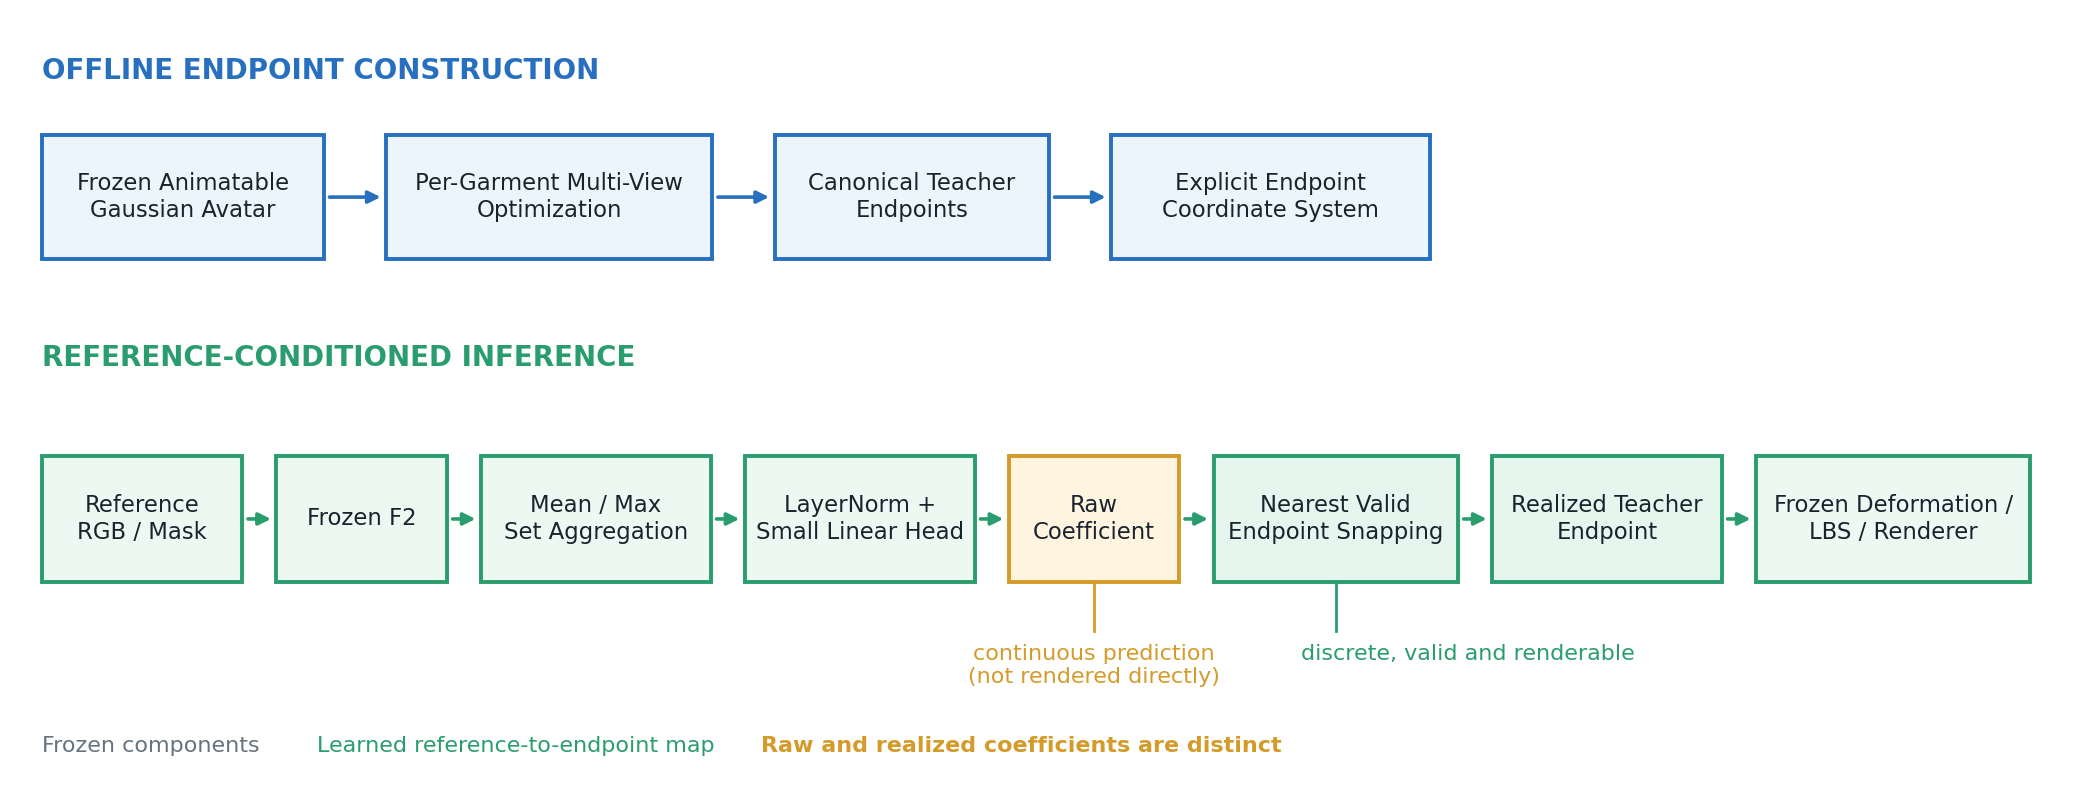
\includegraphics[width=\textwidth]{figures/figure2_canondressgs_pipeline.pdf}
    }{
        \figureplaceholder{0.18\textheight}
        {Figure 2 Placeholder: \method{} Pipeline}
        {\textbf{Offline:} frozen base avatar $\rightarrow$ per-garment multi-view optimization $\rightarrow$ Teacher Endpoints $\rightarrow$ explicit endpoint coordinate system.\\
        \textbf{Inference:} reference RGB/mask $\rightarrow$ frozen F2 features $\rightarrow$ mean/max aggregation $\rightarrow$ LayerNorm $+$ Linear head $\rightarrow$ raw coefficient $\rightarrow$ nearest valid endpoint snapping $\rightarrow$ frozen deformation and rendering.\\
        Mark frozen, trainable, offline-only, and inference-only modules explicitly.}
    }
    \caption{
    \textbf{Overview of \method{}.}
    Garment-specific Teacher Endpoints are optimized in the canonical space of a
    frozen avatar. A lightweight reference branch predicts endpoint-space
    coefficients, after which nearest-endpoint snapping realizes a valid canonical
    state. The target pose and camera enter only the frozen deformation and rendering
    stages. The \dual{} extension is evaluated separately for oracle/user-specified
    endpoint pairs and weights.
    }
    \label{fig:pipeline}
\end{figure*}

\subsection{Problem Setting}

Let the frozen canonical avatar be
\begin{equation}
\mathcal{G}^{0}
=
\left\{
(\mathbf{x}_{i},\mathbf{s}_{i},\mathbf{q}_{i},
 o_{i},\mathbf{h}_{i})
\right\}_{i=1}^{N},
\end{equation}
where $\mathbf{x}_{i}$, $\mathbf{s}_{i}$, $\mathbf{q}_{i}$, $o_i$, and $\mathbf{h}_i$ denote position, scale, rotation, opacity logit, and spherical-harmonic appearance.
The avatar backbone provides a frozen deformation operator $\mathcal{D}$ and renderer $\mathcal{R}$.

For a garment reference set
\begin{equation}
\mathcal{S}
=
\{(I_k,M_k)\}_{k=1}^{K},
\end{equation}
where $I_k$ and $M_k$ are a reference RGB image and garment mask, our goal is to render the fixed identity under target pose $\boldsymbol{\theta}_t$ and camera $\mathcal{C}_t$ while matching the garment specified by $\mathcal{S}$.
The current verified setting is a closed wardrobe of seen garment endpoints.
Target RGB, target mask, target pose, target camera, garment identity, and Teacher residuals do not enter the reference predictor.

\subsection{Canonical Teacher Endpoints}

For each garment $g$, we optimize a canonical residual
\begin{equation}
\Delta\mathcal{G}_{g}
=
\left\{
\Delta\mathbf{x}_{i},
\Delta\log\mathbf{s}_{i},
\Delta\mathbf{r}_{i},
\Delta o_{i},
\Delta\mathbf{h}_{i}
\right\}_{i=1}^{N},
\end{equation}
which is shared across the garment's registered multi-view observations.
To keep the objective within one column, we first define the rendered observation
\begin{equation}
\widehat{I}_{g,v}
=
\mathcal{R}
\left(
\mathcal{D}
\left(
\mathcal{G}^{0}\oplus\Delta\mathcal{G}_{g},
\boldsymbol{\theta}_{g,v}
\right),
\mathcal{C}_{g,v}
\right).
\label{eq:teacher_render}
\end{equation}
The Teacher Endpoint is then
\begin{align}
\Delta\mathcal{G}_{g}^{*}
=
\arg\min_{\Delta\mathcal{G}_{g}}
\sum_{v\in\mathcal{V}_{g}}
\Big[
&\mathcal{L}_{\mathrm{img}}
\left(
\widehat{I}_{g,v},I_{g,v},M_{g,v}
\right)
\nonumber\\[-1mm]
&+\lambda_{\mathrm{reg}}
\mathcal{L}_{\mathrm{reg}}
\left(\Delta\mathcal{G}_{g}\right)
\Big].
\label{eq:teacher_endpoint}
\end{align}
All avatar, deformation, and rendering parameters remain frozen.
The optimized residual is not a ground-truth garment mesh; it is a valid canonical Gaussian state under the frozen avatar representation.

\subsection{Explicit Endpoint Coordinate System}

Given $G$ Teacher Endpoints, we compute their mean
\begin{equation}
\boldsymbol{\mu}
=
\frac{1}{G}
\sum_{g=1}^{G}
\Delta\mathcal{G}_{g}^{*}
\end{equation}
and form the centered endpoint matrix
\begin{equation}
\mathbf{H}
=
\left[
\Delta\mathcal{G}_{1}^{*}-\boldsymbol{\mu},
\ldots,
\Delta\mathcal{G}_{G}^{*}-\boldsymbol{\mu}
\right].
\end{equation}
For the singular-value decomposition $\mathbf{H}=\mathbf{U}\boldsymbol{\Sigma}\mathbf{V}^{\top}$, the rank-$r$ coordinate basis is
\begin{equation}
\mathbf{B}=\mathbf{U}_{[:,1:r]},
\qquad
\mathbf{c}_{g}
=
\mathbf{B}^{\top}
\left(
\Delta\mathcal{G}_{g}^{*}-\boldsymbol{\mu}
\right).
\end{equation}
For subject02, $G=5$ and the maximum centered affine rank is four, so we use $r=4$.
This basis is an explicit endpoint coordinate system, not a strongly compressed universal garment manifold.
Its coordinates are projections of full garment-dependent residual fields rather than arbitrary class codes, so distances organize joint changes in geometry, visibility, and appearance within the closed wardrobe.
Its main value is that it provides a common representation for reference prediction, endpoint realization, analysis, and controlled composition; membership in its affine span alone, however, does not certify a renderable intermediate garment.

\subsection{Reference Feature Aggregation}

A frozen image backbone extracts one feature $\mathbf{f}_{k}\in\mathbb{R}^{256}$ from each clothing-masked reference.
We form the permutation-invariant set representation
\begin{align}
\mathbf{z}_{\mathcal{S}}
=
\Big[
&\operatorname{Mean}_{k}(\mathbf{f}_{k});
\operatorname{Max}_{k}(\mathbf{f}_{k})
\Big]
\in\mathbb{R}^{512}.
\end{align}
The combination of mean and max pooling retains both stable set-level evidence and a strong garment-specific response.
A lightweight endpoint head predicts standardized endpoint coordinates
\begin{equation}
\widehat{\widetilde{\mathbf{c}}}
=
\mathbf{W}\operatorname{LN}
\left(\mathbf{z}_{\mathcal{S}}\right)
+
\mathbf{b}.
\end{equation}
Using frozen normalization statistics computed over the five closed-wardrobe endpoint coefficients, we standardize every raw endpoint coordinate as
\begin{equation}
\widetilde{\mathbf{c}}_{g}
=
(\mathbf{c}_{g}-\mathbf{m}_{c})\oslash\mathbf{s}_{c},
\end{equation}
and optimize coefficient SmoothL1 only,
\begin{equation}
\mathcal{L}_{\mathrm{ctrl}}
=
\frac{1}{r}\sum_{j=1}^{r}
\operatorname{SmoothL1}
\left(
\widehat{\widetilde{c}}_{j}-\widetilde{c}_{g,j};\,\beta=1
\right).
\end{equation}
No classification, rendering, or pairwise-geometry loss is used.
For subject02, the head outputs four coefficients and has 3,076 trainable parameters; it is trained for 300 Adam steps with learning rate 0.02 while the image backbone, basis, avatar, deformation model, and renderer remain frozen.

\subsection{Nearest-Valid-Endpoint Realization}

Raw coefficient prediction is not required to reconstruct a physically meaningful intermediate garment.
Instead, we identify the closest valid endpoint:
\begin{align}
\widehat{g}
&=
\arg\min_{g}
\left\|
\widehat{\widetilde{\mathbf{c}}}-\widetilde{\mathbf{c}}_{g}
\right\|_{2},
\\
\mathbf{c}_{\mathrm{realized}}
&=
\mathbf{c}_{\widehat{g}}.
\end{align}
The realized residual is
\begin{equation}
\Delta\mathcal{G}_{\mathrm{realized}}
=
\boldsymbol{\mu}
+
\mathbf{B}\mathbf{c}_{\mathrm{realized}}.
\end{equation}
The final target rendering is
\begin{align}
\widehat{I}_{t}
=
\mathcal{R}
\Big(
\mathcal{D}
\big(
&\mathcal{G}^{0}\oplus
\Delta\mathcal{G}_{\mathrm{realized}},
\boldsymbol{\theta}_{t}
\big),
\mathcal{C}_{t}
\Big).
\end{align}
This explicitly distinguishes the \emph{raw predicted coefficient} from the \emph{realized snapped coefficient}.
The predictor therefore estimates a location in a structured residual coordinate system rather than outputting a garment class directly.
For the deployed closed-wardrobe path, it only needs to place the reference inside the correct endpoint region; snapping then projects that estimate onto the verified set of optimized garment states.

\subsection{Geometry-Safe Dual-Support Extension}

For two valid endpoints $a$ and $b$, direct interpolation constructs
\begin{equation}
\mathcal{G}_{\mathrm{lin}}(\alpha)
=
(1-\alpha)\mathcal{G}_{a}
+
\alpha\mathcal{G}_{b},
\end{equation}
which linearly moves, rescales, and rotates Gaussian geometry.
Even when both endpoints are valid, the intermediate support may not correspond to a valid garment.

\dual{} instead keeps two immutable endpoint geometries.
For user-specified or oracle weights $w_a$ and $w_b$, it scales the effective opacity of each endpoint:
\begin{equation}
\widetilde{\alpha}_{g,i}
=
w_g\,\sigma(o_{g,i}),
\qquad
g\in\{a,b\},
\end{equation}
and renders the union
\begin{equation}
\mathcal{G}_{\mathrm{DS}}
=
\mathcal{G}_{a}^{w_a}
\cup
\mathcal{G}_{b}^{w_b}.
\end{equation}
No interpolation is applied to $\mathbf{x}$, $\mathbf{s}$, or $\mathbf{q}$.
Appearance remains attached to its corresponding endpoint geometry.
The current verified \dual{} evaluation uses oracle or user-specified endpoint pairs and weights; automatic mixed-reference routing is not part of the claimed method.

\section{Experiments}

\subsection{Questions}

We organize the experiments around five questions:
\begin{itemize}
    \item \textbf{Q1:} Can valid garment endpoints be constructed on a frozen animatable avatar?
    \item \textbf{Q2:} Can references reliably realize the correct endpoint without garment identity?
    \item \textbf{Q3:} Which reference-conditioning and realization designs are necessary?
    \item \textbf{Q4:} Why does direct geometry interpolation fail, and does \dual{} improve controlled intermediate states?
    \item \textbf{Q5:} Does the same endpoint-editing pipeline replicate on a second identity?
\end{itemize}

\subsection{Datasets and Protocol}

The primary benchmark uses THuman4.0 subject02 with five preregistered seen garments: O01, O02, O03, O04, and O08.
Teacher optimization, reference prediction, target rendering, and evaluation use frozen manifests and condition-fold cross-validation.
Each of four rotations uses two conditions for training, one for calibration, and one for testing.
With three seeds, this gives 12 \method{} controller runs and 12 matched classifier runs, or 24 optimizer runs in total; the primary clean denominator is 60 unique queries per evaluated method.

We additionally include a second-identity replication on THuman4.0 subject00.
The frozen plan uses garments O01, O03, and O04.
Subject00 will construct three Teacher Endpoints, a rank-$\leq 2$ endpoint coordinate system, a subject-specific reference controller with the same architecture and hyperparameters, hard-lookup baselines, and identity-safety evaluation.
The concrete Subject00 values are intentionally blank in this draft pending completion of the sealed formal base, garment data generation, endpoint construction, and controller evaluation.

\begin{table}[t]
\centering
\small
\caption{Benchmark scope. Subject00 values remain blank until the second-identity experiment is sealed.}
\label{tab:benchmark}
\resizebox{\columnwidth}{!}{%
\begin{tabular}{@{}lccccc@{}}
\toprule
Identity & Garments & Endpoint rank & \method{} runs & Clean queries & Status\\
\midrule
subject02 & 5 & 4 & 12 & 60 & complete\\
subject00 & 3 & $\leq 2$ & \pending & \pending & pending\\
\bottomrule
\end{tabular}%
}
\end{table}

\subsection{Baselines}

We compare methods that isolate different aspects of the problem:
\begin{itemize}
    \item \textbf{Base Avatar:} applies no garment residual.
    \item \textbf{Teacher Endpoint:} directly uses the optimized target endpoint and serves as a non-deployable representation upper bound.
    \item \textbf{Outfit-ID Oracle Lookup:} retrieves the correct endpoint using privileged garment identity.
    \item \textbf{Linear Coefficient Predictor:} uses the same reference features, head, loss, and training schedule as \method{}, but renders the de-standardized raw coefficient without nearest-endpoint projection.
    \item \textbf{Reference Classifier Lookup:} classifies the reference into one of the seen garments and retrieves the corresponding endpoint.
    \item \textbf{Nearest-Centroid Lookup:} retrieves the endpoint whose frozen feature centroid is closest to the reference.
    \item \textbf{Linear Geometry Interpolation:} directly interpolates all Gaussian endpoint attributes.
    \item \textbf{Hard Geometry:} selects one endpoint geometry and therefore does not form a true intermediate state.
    \item \textbf{\dual{}:} preserves two endpoint geometries and weights their effective opacity.
\end{itemize}

Earlier global-feature, mean-only, legacy-supervision, and dense-decoder experiments used a different exploratory protocol and are not pooled into the current cross-fit table.
In particular, the historical dense decoder covers only O01/O08 and never completed its reference-conditioned stage, while the historical ``Legacy Endpoint'' label was found to be contract-ambiguous.
We retain those experiments as diagnostic provenance rather than present their unmatched metrics as formal baselines.

\subsection{Closed-Wardrobe Endpoint Editing}

Across 12 \method{} cross-fit runs, the 60-query clean evaluation obtains top-1 accuracy of 1.0.
Every garment attains precision and recall of 1.0, endpoint exact match is 1.0, identity and component contamination are both zero, and no severe wrong-outfit failure is observed.
The deployed reference path therefore matches the correct Teacher Endpoint without using privileged garment identity.

\begin{table*}[t]
\centering
\small
\caption{Closed-wardrobe endpoint selection, realization, and robustness on subject02. Results use 60 unique queries per evaluated method and perturbation. ``Clean top-1/exact'' separates selection of the correct endpoint region from exact coefficient realization. Endpoint RGB MAE and LPIPS compare a realized render with its corresponding Teacher Endpoint and therefore measure realization parity, not Teacher quality. Values marked with $\dagger$ use privileged information or direct optimization; dashes denote undefined metrics.}
\label{tab:endpoint_main}
\resizebox{\textwidth}{!}{%
\begin{tabular}{@{}lccccccc@{}}
\toprule
Method & Ref. only & Clean top-1/exact$\uparrow$ & Endpoint RGB MAE$\downarrow$ & Endpoint LPIPS$\downarrow$ & Blur top-1$\uparrow$ & 1-ref top-1$\uparrow$ & Params.\\
\midrule
Base Avatar & no & --/-- & 0.247505309 & 0.121243553 & -- & -- & 0\\
Teacher Endpoint$^{\dagger}$ & no & --/-- & 0 & 0 & -- & -- & 0\\
Outfit-ID Oracle Lookup$^{\dagger}$ & no & 1.000/1.000 & $9.288668\times10^{-7}$ & $3.191450\times10^{-7}$ & -- & -- & 0\\
\midrule
Reference Classifier Lookup & yes & 1.000/1.000 & $9.288668\times10^{-7}$ & $3.191450\times10^{-7}$ & \textbf{0.516667} & \textbf{1.000} & 3,589\\
Nearest-Centroid Lookup & yes & 1.000/1.000 & $9.288668\times10^{-7}$ & $3.191450\times10^{-7}$ & 0.300000 & 0.900 & 0\\
\midrule
Linear Coefficient Predictor & yes & 1.000/0.000 & 0.053906807 & 0.067913007 & 0.350000 & 0.950 & 3,076\\
\textbf{\method{}} & yes & 1.000/1.000 & $9.288668\times10^{-7}$ & $3.191450\times10^{-7}$ & 0.350000 & 0.950 & 3,076\\
\bottomrule
\end{tabular}%
}
\end{table*}

The classifier and centroid baselines saturate the clean five-garment classification task.
This result does not make the proposed representation redundant.
The clean result is therefore a disclosed functional equivalence, not a superiority claim over hard lookup.
The distinction appears between prediction and realization: the unsnapped coefficient baseline reaches the same 1.0 top-1 accuracy but has zero exact endpoint matches, coefficient MAE 71.4451, RGB MAE 0.053907, and endpoint LPIPS 0.067913.
Projection changes only the realized state, giving exact match 1.0, RGB MAE $9.29\times10^{-7}$, and endpoint LPIPS $3.19\times10^{-7}$.
The coordinate representation remains useful because it supports this valid-state projection, distance-based diagnostics, and the geometry-safe composition operator studied below.



\subsection{Reference Conditioning and Snapping}

Because the linear coefficient baseline and \method{} share the same features, head, loss, and training schedule, their difference isolates nearest-valid-state projection.
The result shows that the head need not solve exact continuous regression: it identifies the correct endpoint basin for all 60 clean queries even though its raw coefficients are not endpoint-exact.
As expected, projection does not alter endpoint routing, so the linear predictor and \method{} have identical perturbation top-1 values.
The reference classifier is more robust to mild blur and a single reference in this experiment (0.516667 and 1.000) than \method{} (0.350000 and 0.950); we therefore make no robustness-superiority claim.

For \method{}, top-1 remains 1.0 under mask erosion, mask dilation, reference assignment permutation, and partial reference dropout; using one reference gives 0.95.
Mild blur is the clear weakness, reducing top-1 to 0.35 and producing a 0.65 endpoint-flip rate.
Complete reference dropout is evaluated separately and safely abstains to the Base Avatar in all 80 registered cases; observed identity contamination remains zero.

\subsection{Geometry Causal Attribution}

We isolate geometry, visibility, and appearance with an endpoint-anchored $2^3$ intervention.
The measured geometry main effect is 0.99594054.
Geometry is sufficient and necessary for failure in all ten unordered garment pairs, whereas visibility and appearance alone are not sufficient.
This supports the design choice of preserving endpoint geometry rather than learning a more complex appearance-only correction.

\begin{table}[t]
\centering
\small
\caption{Causal attribution over all ten subject02 garment pairs.}
\label{tab:causal}
\resizebox{\columnwidth}{!}{%
\begin{tabular}{@{}lccc@{}}
\toprule
Factor & Main effect & Sufficient & Necessary\\
\midrule
Geometry & \textbf{0.9959} & \textbf{10/10} & \textbf{10/10}\\
Visibility & 0.0129 & 0/10 & 0/10\\
Appearance & 0.0324 & 0/10 & 0/10\\
\bottomrule
\end{tabular}%
}
\end{table}

% --------------------------------------------------------------------------
% Figure 3: Geometry-causal evidence.
% Expected file: figures/figure3_geometry_causal_analysis.pdf
% --------------------------------------------------------------------------
\begin{figure*}[t]
    \centering
    \IfFileExists{figures/figure3_geometry_causal_analysis.pdf}{
        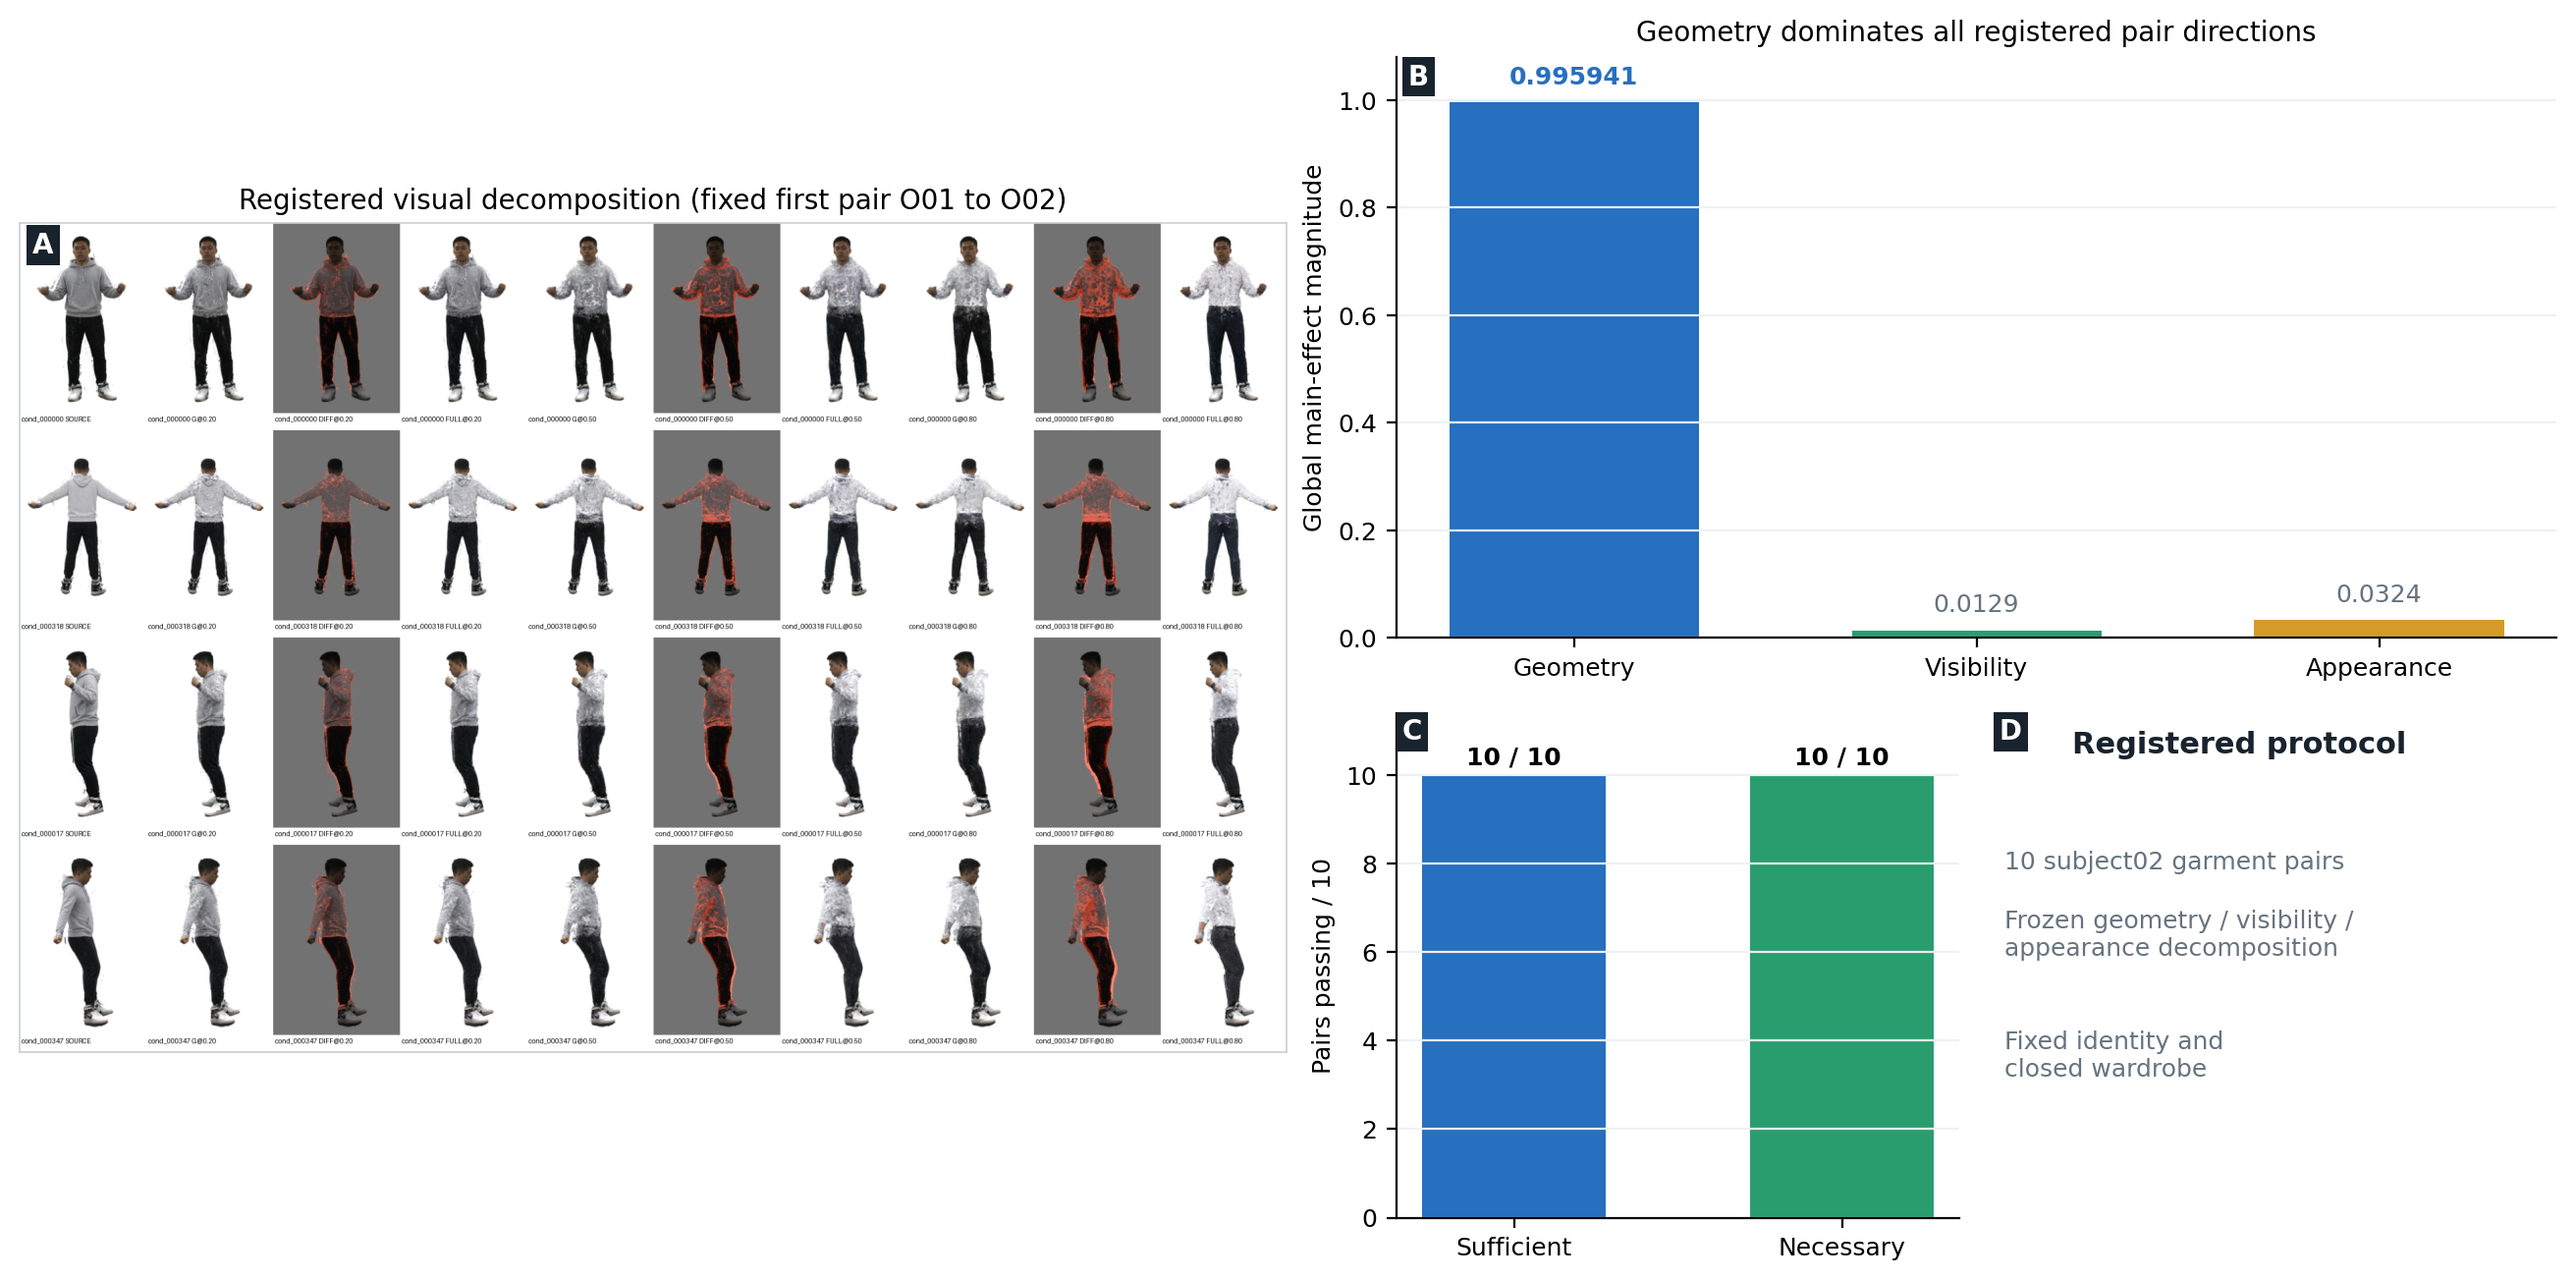
\includegraphics[width=\textwidth]{figures/figure3_geometry_causal_analysis.pdf}
    }{
        \figureplaceholder{0.18\textheight}
        {Figure 3 Placeholder: Geometry-Causal Analysis}
        {Suggested layout: endpoint A; linear intermediate; endpoint B; geometry-only intervention; visibility-only intervention; appearance-only intervention; aggregate main effects; sufficient/necessary counts.\\
        Include representative cloud, mottle, edge-scatter, and silhouette failures using unchanged scientific pixels.}
    }
    \caption{
    \textbf{Why direct endpoint interpolation fails.}
    Endpoint-anchored interventions show that interpolated Gaussian geometry is the
    dominant cause of invalid intermediate states. Geometry is sufficient and
    necessary for the failure across all ten garment pairs, motivating endpoint
    snapping and geometry-preserving composition.
    }
    \label{fig:geometry_causal}
\end{figure*}

\subsection{Geometry-Safe Intermediate States}

Table~\ref{tab:dual} compares three internal mechanisms.
Linear geometry interpolation forms a continuous coefficient path but moves Gaussian supports through invalid states.
Hard geometry obtains a low perceptual distance by selecting one endpoint, but it performs a discrete switch rather than a genuine composition.
\dual{} preserves both endpoint geometries and provides a weighted intermediate rendering.

\begin{table}[t]
\centering
\small
\setlength{\tabcolsep}{3.5pt}
\caption{Verified all-pair mechanism comparison on subject02. \dual{} uses oracle or user-specified endpoint pairs and weights.}
\label{tab:dual}
\resizebox{\columnwidth}{!}{%
\begin{tabular}{@{}lcccc@{}}
\toprule
Method & LPIPS$\downarrow$ & IoU$\uparrow$ & Boundary F$\uparrow$ & Geometry support\\
\midrule
Linear geometry & 0.0853 & 0.7101 & 0.3003 & interpolated\\
Hard geometry & \textbf{0.0318} & 0.7120 & 0.3689 & one endpoint\\
\dual{} & 0.0570 & \textbf{0.7253} & \textbf{0.3791} & two endpoints\\
\bottomrule
\end{tabular}%
}
\end{table}

Relative to linear geometry interpolation, \dual{} improves LPIPS from 0.085303 to 0.056985, IoU from 0.710052 to 0.725290, and Boundary F from 0.300263 to 0.379103.
Severe artifacts improve for all ten garment pairs and identity contamination remains zero.
The cost is approximately twice as many active Gaussians and 1.626$\times$ rendering time in dual mode.
This is a favorable quality--cost trade-off for controlled composition, but it is not yet an automatic mixed-reference system.

% --------------------------------------------------------------------------
% Figure 4: All-pair Dual-Support comparison.
% Expected file: figures/figure4_dual_support_all_pair.pdf
% --------------------------------------------------------------------------
\begin{figure*}[t]
    \centering
    \IfFileExists{figures/figure4_dual_support_all_pair.pdf}{
        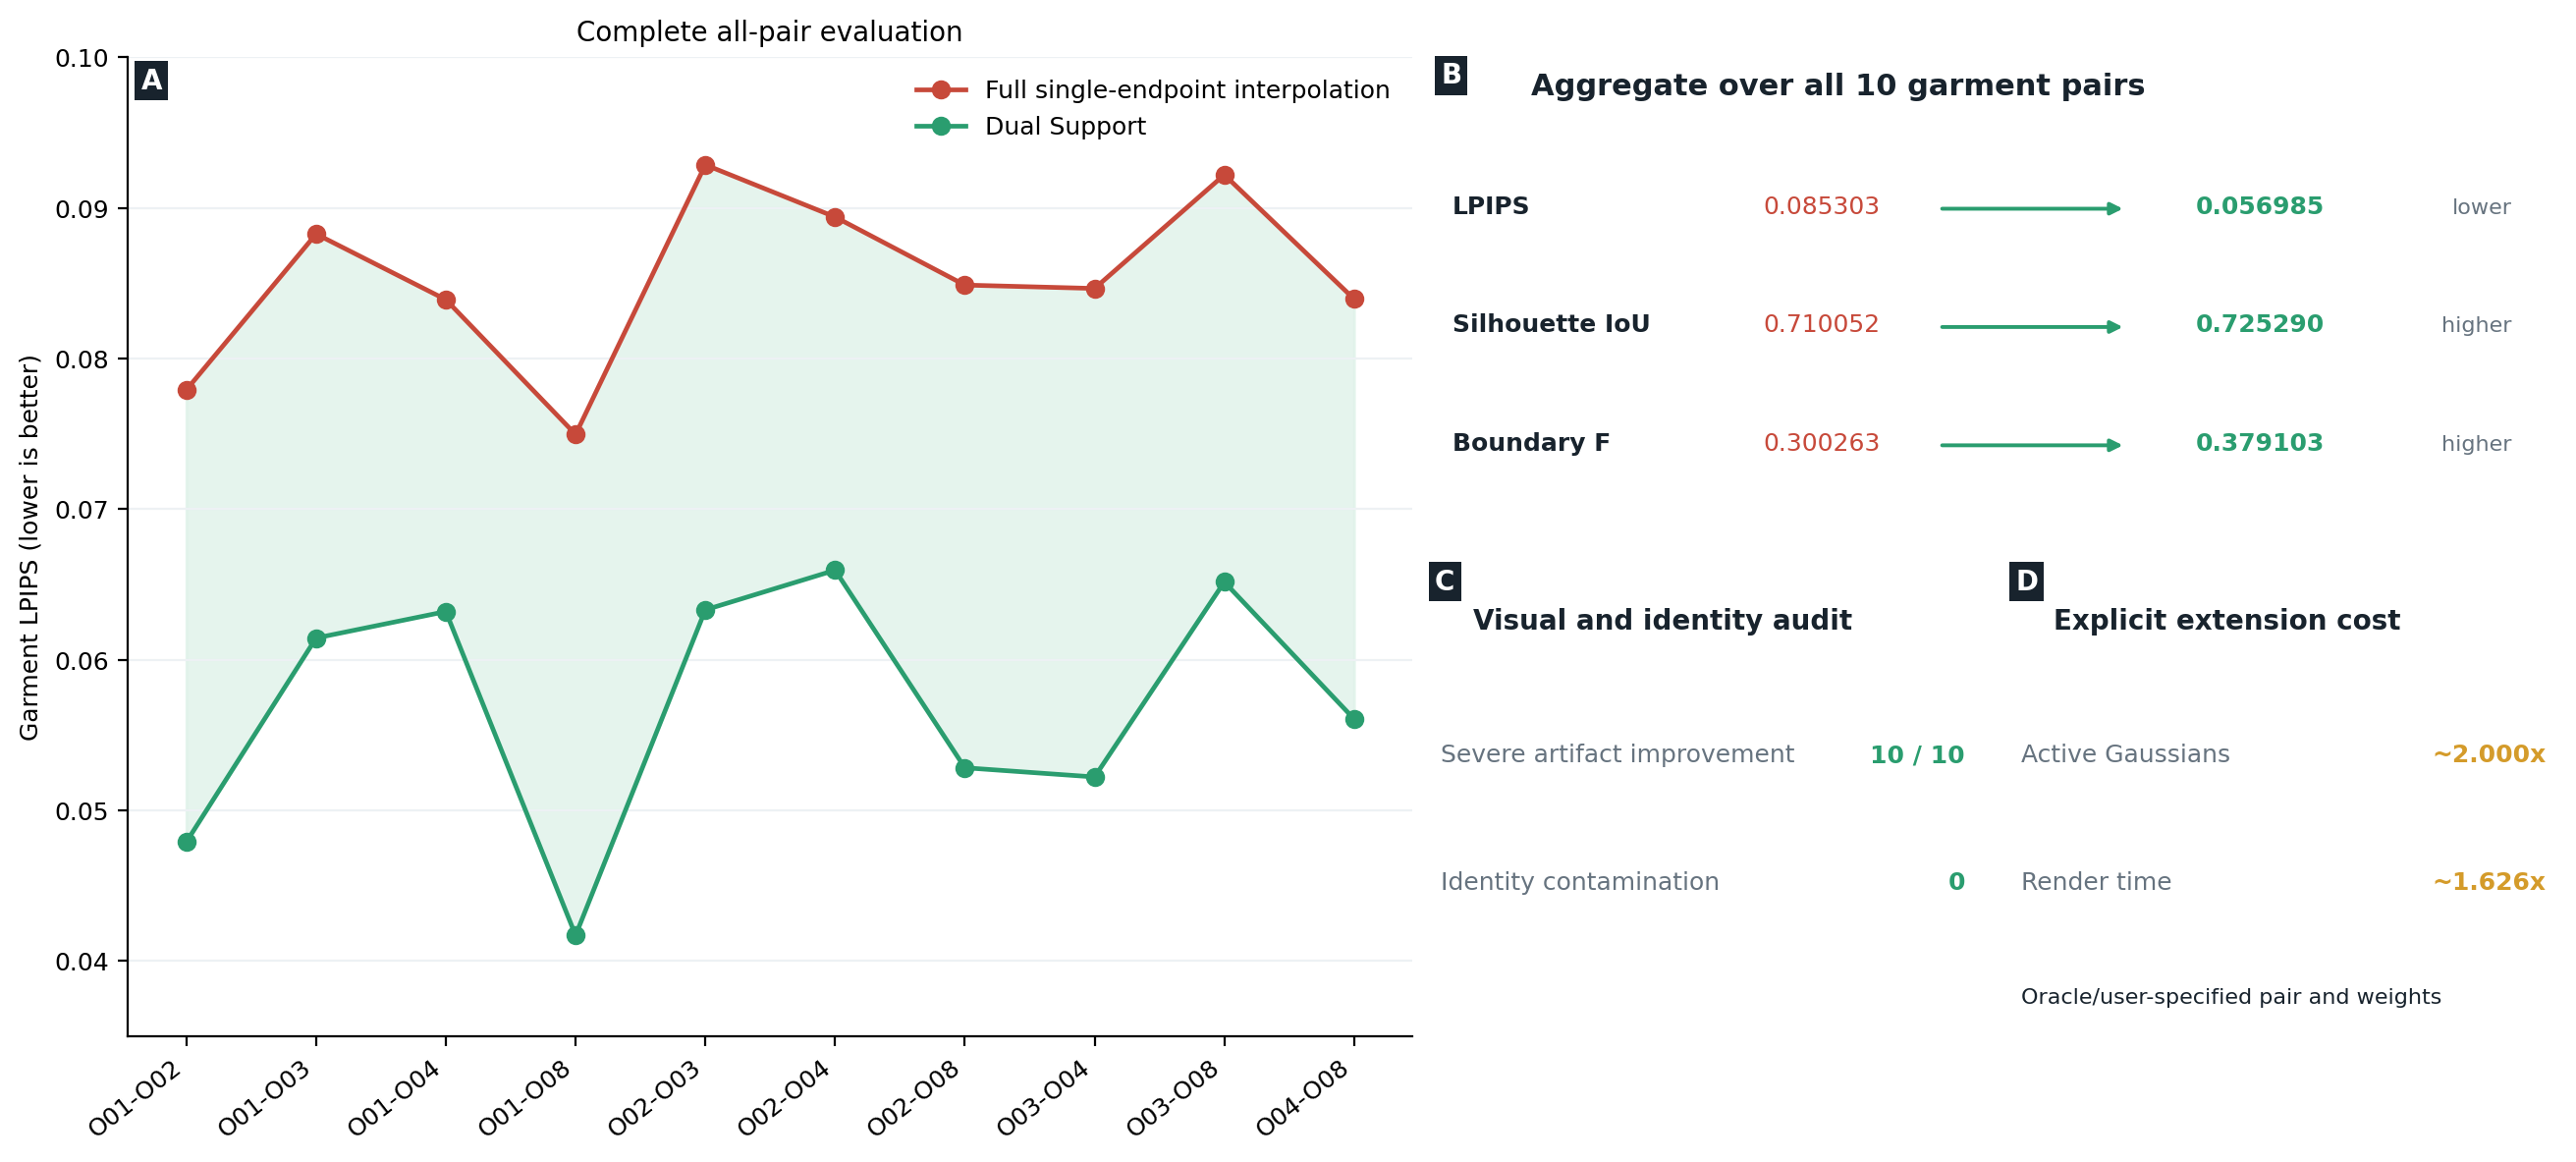
\includegraphics[width=\textwidth]{figures/figure4_dual_support_all_pair.pdf}
    }{
        \figureplaceholder{0.19\textheight}
        {Figure 4 Placeholder: Geometry-Safe Intermediate States}
        {Columns: endpoint A; 20\%; 50\%; 80\%; endpoint B.\\
        Rows: linear geometry interpolation; hard geometry; oracle/user-specified \dual{}.\\
        Include at least one strong pair and the difficult O01--O03 or O02--O03 pair, plus an all-pair quantitative summary and the $2\times$ Gaussian / $1.626\times$ runtime cost.}
    }
    \caption{
    \textbf{Intermediate garment states.}
    Linear interpolation moves Gaussian geometry through unsupported configurations.
    Hard geometry switches discretely to one endpoint. \dual{} retains two valid
    endpoint supports and weights their effective opacity, improving perceptual and
    boundary quality while exposing the additional runtime cost.
    }
    \label{fig:dual_support}
\end{figure*}

% --------------------------------------------------------------------------
% Figure 5: Hard-lookup relation and raw-versus-snapped endpoint realization.
% Expected file: figures/figure5_hard_lookup_relation.pdf
% --------------------------------------------------------------------------
\begin{figure*}[t]
    \centering
    \IfFileExists{figures/figure5_hard_lookup_relation.pdf}{
        
\includegraphics[width=\textwidth]{figures/figure5_hard_lookup_relation.pdf}
    }{
        \figureplaceholder{0.17\textheight}
        {Figure 5 Placeholder: Endpoint Prediction, Snapping, and Hard Lookup}
        {Suggested panels: raw coefficient location; nearest endpoint; realized snapped coefficient; rendered parity with the corresponding Teacher Endpoint; clean agreement with classifier/centroid lookup; representative perturbation disagreement cases.\\
        The figure must state that clean closed-bank renders are functionally equivalent when all methods select the same endpoint.}
    }
    \caption{
    \textbf{Relation to hard lookup and the role of snapping.}
    Clean classifier, centroid, and \method{} predictions may select the same
    endpoint and therefore produce equivalent renders. The explicit coefficient
    prediction remains useful for structured endpoint-space analysis, while snapping
    converts an approximate raw prediction into an exact valid garment realization.
    }
    \label{fig:hard_lookup}
\end{figure*}

\subsection{Comparison with Prior Intermediate-State Methods}

The final submission should include matched comparisons with prior controllable Gaussian, avatar blend-space, or garment interpolation methods.
A fair comparison must use the same endpoint pairs, target views, masks, and evaluation regions, and should report:
\begin{itemize}
    \item intermediate-state LPIPS, silhouette IoU, and Boundary F;
    \item severe cloud, mottle, edge-scatter, and double-outline counts;
    \item active Gaussian count, storage, and rendering time;
    \item whether the method requires per-pair retraining, a garment mesh, simulation, or additional topology;
    \item whether endpoint geometry remains valid throughout the path.
\end{itemize}
No cross-paper superiority claim is made in this draft before these matched evaluations are completed.
The current verified claim is that \dual{} is substantially better than direct Gaussian geometry interpolation and offers a lightweight runtime operator relative to retraining a new dense residual field for every mixture.

\subsection{Representation Scope}

The explicit coordinate system is more expressive than a bare class lookup because it supports coefficient-valued states, distance-based analysis, and composition operators.
However, the current global affine basis does not yet yield reliable arbitrary intermediate garments.
Test-time coefficient refinement does not improve over the Teacher Endpoint: Teacher LPIPS is 0.038768 and refined LPIPS is 0.038982, with zero of five garments meeting the improvement threshold; equal-step full-residual optimization is worse at 0.118421 LPIPS.
Leave-one-garment-out evaluation further shows that a rank-3 basis constructed from four garments has insufficient capacity for reliable adaptation to the fifth garment: zero of five folds passes the capacity criterion, while low-dimensional adaptation and nearest hard lookup obtain similarly poor LPIPS values of 0.113551 and 0.113437.
We therefore interpret the current basis as an endpoint-centered editing representation, not as a universal open-set garment manifold.

% --------------------------------------------------------------------------
% Figure 6: Headroom, LOO, perturbation, and fallback scope analysis.
% Expected file: figures/figure6_scope_analysis.pdf
% --------------------------------------------------------------------------
\begin{figure*}[t]
    \centering
    \IfFileExists{figures/figure6_scope_analysis.pdf}{
        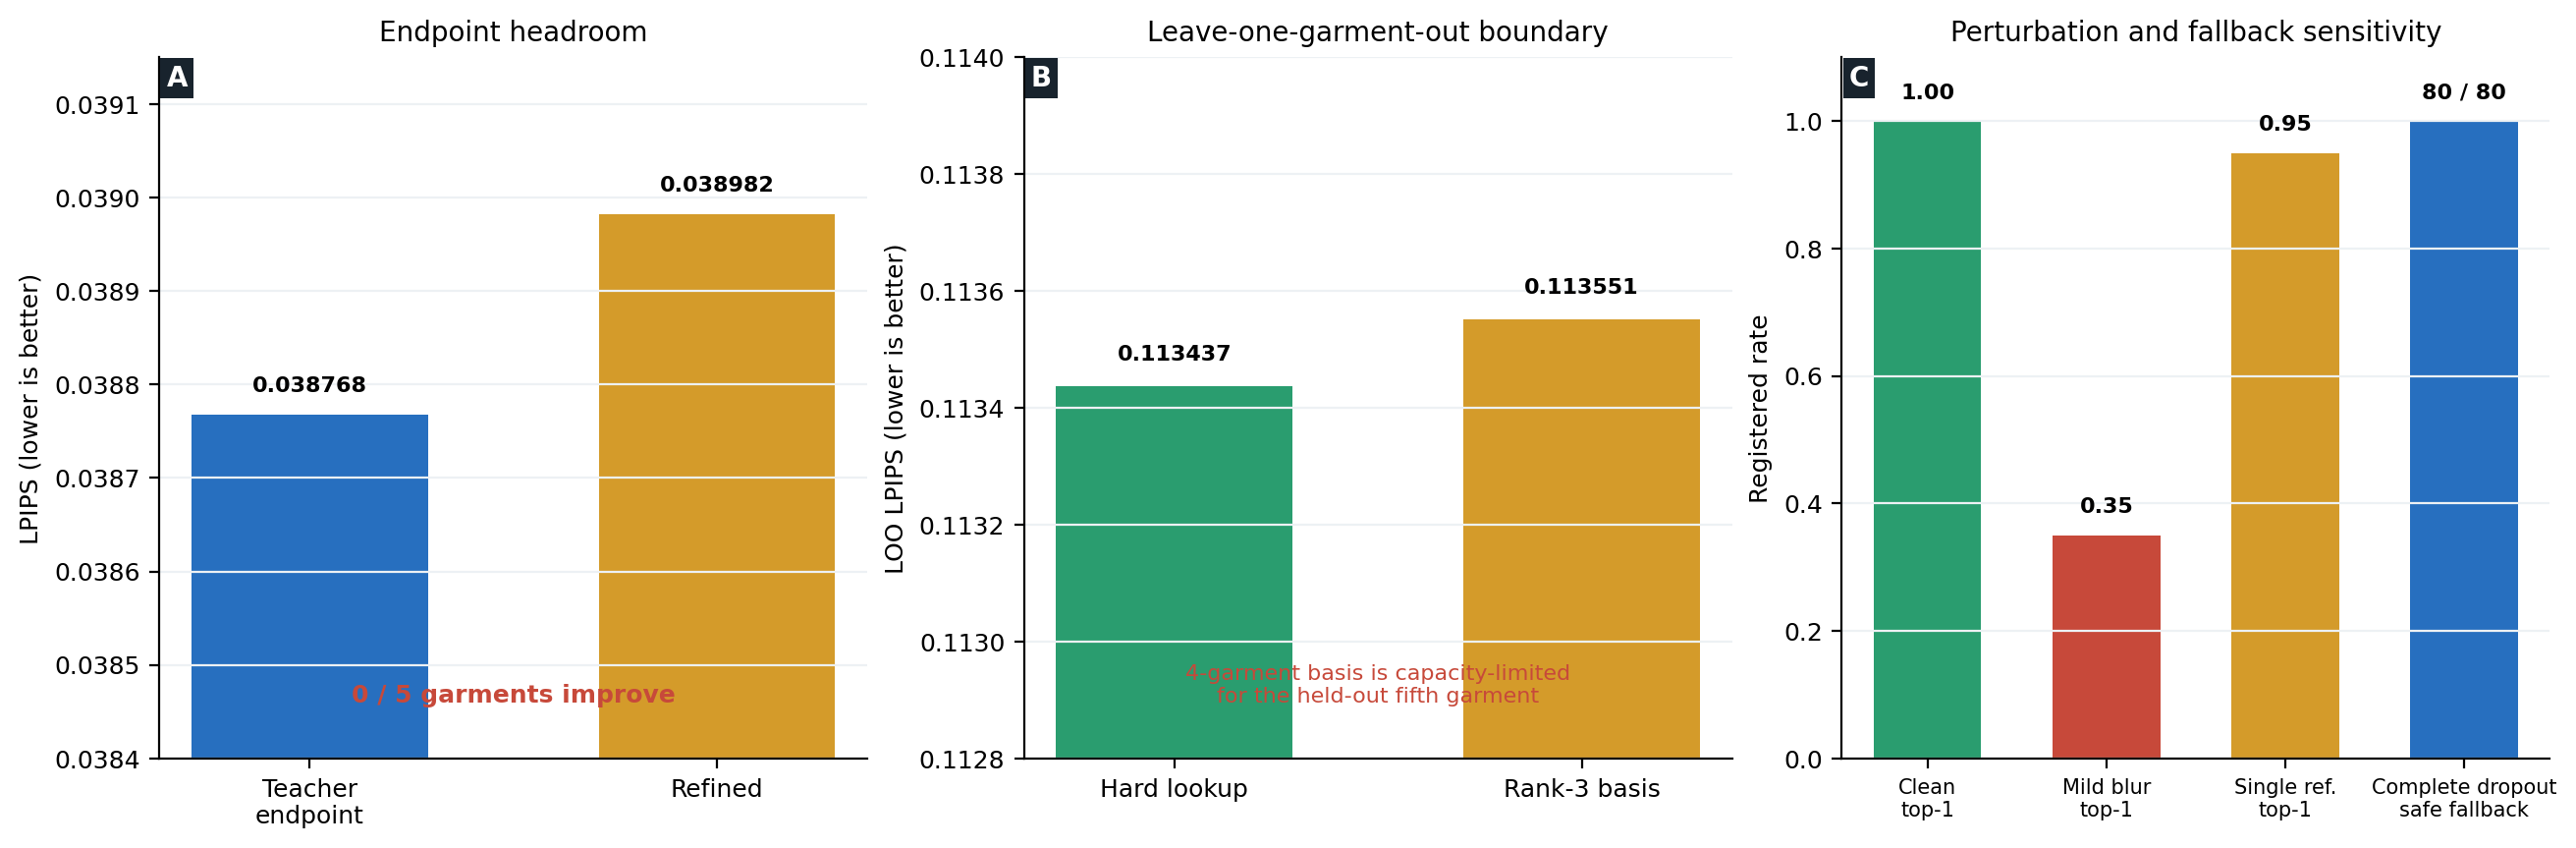
\includegraphics[width=\textwidth]{figures/figure6_scope_analysis.pdf}
    }{
        \figureplaceholder{0.18\textheight}
        {Figure 6 Placeholder: Representation Scope and Failure Boundaries}
        {Suggested panels: Teacher-versus-refined LPIPS; five LOO folds; raw-versus-snapped coefficient error; single-reference robustness; mild-blur endpoint flips; complete-dropout safe fallback.\\
        Present Headroom and LOO as scope analyses, not as the primary method result.}
    }
    \caption{
    \textbf{Scope of the current endpoint representation.}
    The rank-4 subject02 coordinate system precisely organizes the five seen
    endpoints, but test-time refinement does not surpass the Teacher states and a
    four-garment rank-3 span does not reliably adapt to a held-out fifth garment.
    Snapping and safe fallback therefore remain essential in the current system.
    }
    \label{fig:scope}
\end{figure*}

\subsection{Second-Identity Replication on Subject00}

Subject00 is included to test whether the endpoint construction and reference-control pipeline can be replicated for a second identity rather than tuned only to subject02.
The protocol fixes garments O01, O03, and O04; constructs three independent Teacher Endpoints; builds a rank-$\leq2$ coordinate system; retrains the same lightweight endpoint head with unchanged design choices; and compares against classifier lookup, nearest-centroid lookup, outfit-ID oracle, and Teacher Endpoints.

\begin{table*}[t]
\centering
\small
\caption{Second-identity replication on subject00. All values are intentionally blank pending the sealed formal base, garment data, Teacher Endpoints, and controller evaluation.}
\label{tab:subject00}
\resizebox{\textwidth}{!}{%
\begin{tabular}{@{}lcccccc@{}}
\toprule
Method & Clean top-1$\uparrow$ & Macro precision$\uparrow$ & Macro recall$\uparrow$ & Exact endpoint$\uparrow$ & Identity contam.$\downarrow$ & LPIPS$\downarrow$\\
\midrule
Base Avatar & \pending & \pending & \pending & \pending & \pending & \pending\\
Reference Classifier Lookup & \pending & \pending & \pending & \pending & \pending & \pending\\
Nearest-Centroid Lookup & \pending & \pending & \pending & \pending & \pending & \pending\\
\method{} & \pending & \pending & \pending & \pending & \pending & \pending\\
Outfit-ID Oracle Lookup$^{\dagger}$ & \pending & \pending & \pending & \pending & \pending & \pending\\
Teacher Endpoint$^{\dagger}$ & \pending & \pending & \pending & \pending & \pending & \pending\\
\bottomrule
\end{tabular}%
}
\end{table*}

The intended conclusion is deliberately limited to second-identity replication.
This experiment will not be described as cross-dataset, unseen-identity, or zero-shot controller transfer.

% --------------------------------------------------------------------------
% Figure 7: Optional subject00 second-identity replication.
% Expected file: figures/figure7_subject00_replication.pdf
% --------------------------------------------------------------------------
\begin{figure*}[t]
    \centering
    \IfFileExists{figures/figure7_subject00_replication.pdf}{
        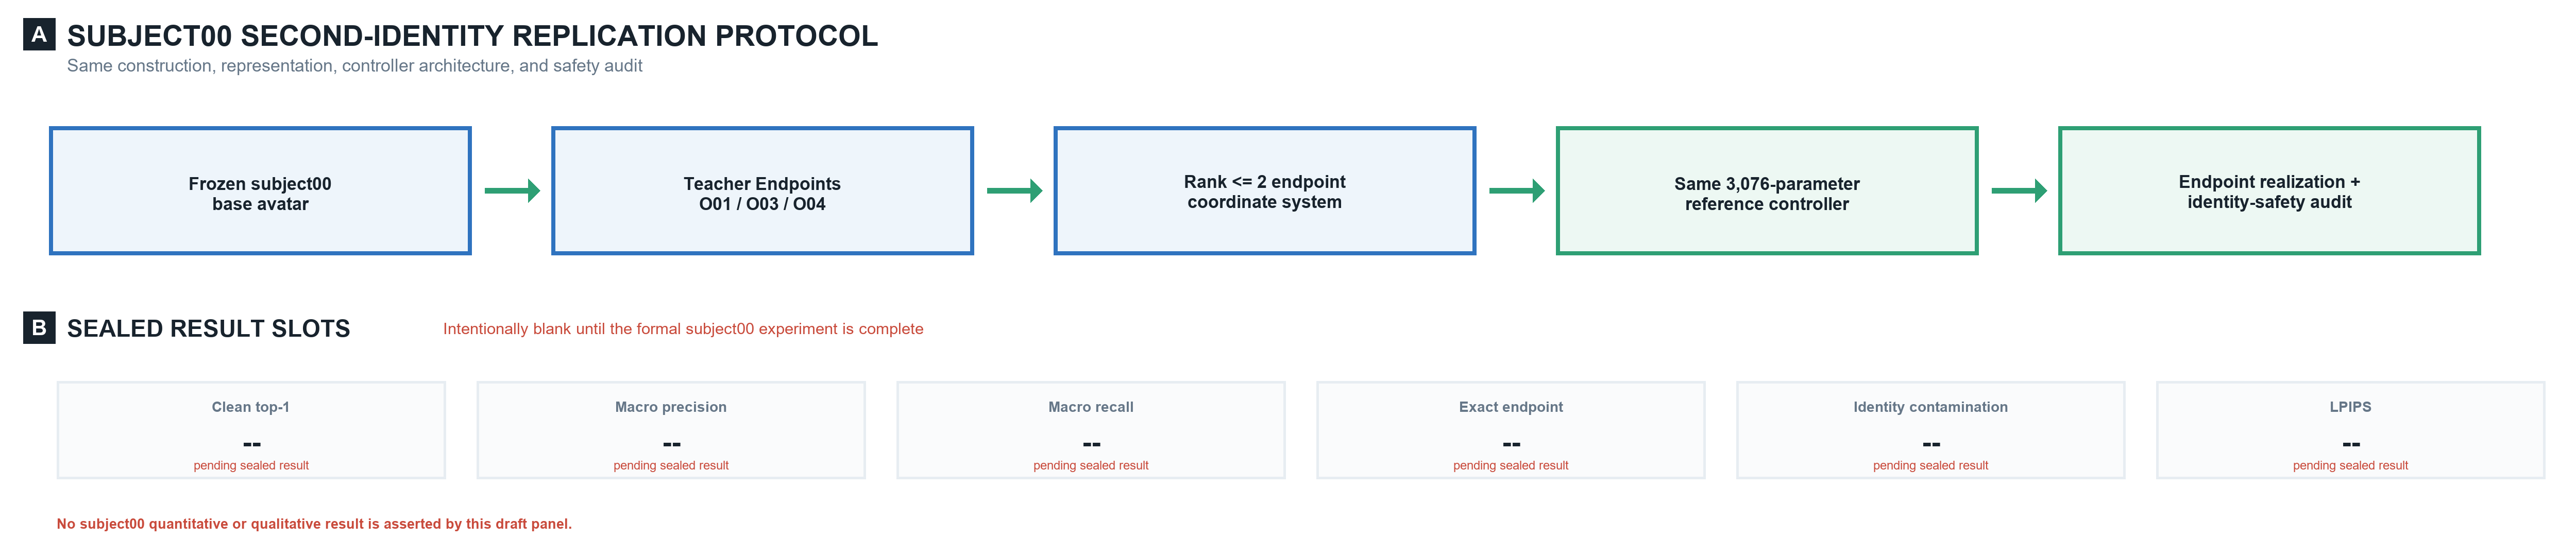
\includegraphics[width=\textwidth]{figures/figure7_subject00_replication.pdf}
    }{
        \figureplaceholder{0.17\textheight}
        {Figure 7 Placeholder: Subject00 Second-Identity Replication}
        {Suggested layout after results are sealed: identity/reference inputs; O01/O03/O04 Teacher Endpoints; classifier lookup; nearest-centroid lookup; \method{}; matched target poses/cameras; identity-preservation crops.\\
        Leave this placeholder in the draft, but remove it from the submission if subject00 remains incomplete or the page budget is exceeded.}
    }
    \caption{
    \textbf{Second-identity replication.}
    The final panel will test whether the same Teacher construction, endpoint-space
    representation, reference head, and snapping rule reproduce on subject00 with
    three garments. No subject00 result is claimed until the formal base and all
    downstream experiments are sealed.
    }
    \label{fig:subject00}
\end{figure*}

\subsection{Qualitative Results}

Figure~\ref{fig:teaser} should provide the task-level visual summary.
Figure~\ref{fig:hard_lookup} should compare reference inputs, Base Avatar, the strongest hard-lookup baseline, raw coefficient rendering, the snapped \method{} result, and the Teacher Endpoint under the same target pose and camera.
Figure~\ref{fig:geometry_causal} should visualize the causal interventions, while Figure~\ref{fig:dual_support} should compare linear geometry, hard geometry, and \dual{} at matched mixture weights.
All five subject02 garments must be represented with consistent views.
Subject00 should appear only after the corresponding sealed results are available.

\section{Limitations}

The present evaluation is a closed wardrobe of seen garments.
Adding a new garment requires multi-view Teacher optimization, updating the endpoint coordinate system, and potentially retraining the lightweight predictor.
The current subject02 evaluation is based on one identity, although a three-garment subject00 replication is planned and explicitly represented in the draft.

Clean endpoint selection is saturated by strong classifier and nearest-centroid lookup baselines.
\method{} therefore does not claim higher clean classification accuracy than every retrieval system.
Its benefit is the complete garment-editing representation: valid Teacher construction, reference-to-coordinate prediction, exact endpoint realization, identity-safe failure behavior, and a geometry-safe composition interface.

The current global affine basis is not sufficient for open-set garment adaptation.
Raw coefficient prediction is less reliable than snapped endpoint realization, mild blur can cause endpoint flips, and automatic mixed-reference pair/weight prediction remains unresolved.
\dual{} currently assumes oracle or user-specified endpoints and weights and costs approximately twice the active Gaussian count and 1.626$\times$ render time.

Finally, the method inherits the spatial support of the frozen avatar.
Garments requiring substantially different topology, thickness, or independently moving cloth may require a separate garment Gaussian layer, adaptive support, or physical simulation.

\section{Conclusion}

We presented \method{}, a geometry-safe reference-controlled garment editing framework for animatable Gaussian avatars.
The method constructs valid canonical Teacher Endpoints on a frozen avatar, organizes them in an explicit endpoint coordinate system, maps garment references to this space with a lightweight predictor, and uses nearest-valid-endpoint snapping for robust realization.
The matched ablation shows that raw coefficient prediction can locate the correct endpoint region without reconstructing a valid endpoint, while nearest-valid-state projection converts that estimate into exact endpoint realization; the separate \dual{} analysis improves over direct geometry interpolation without moving Gaussian geometry between endpoints.
On a five-garment subject02 wardrobe, it achieves perfect clean endpoint selection, exact Teacher realization, zero identity contamination, and no severe wrong-outfit failures, while matching saturated classifier and centroid lookup without privileged garment identity.

The explicit representation is broader than a bare lookup table because it supports coefficient-valued analysis and geometry-aware composition.
At the same time, our experiments show that arbitrary global-basis interpolation is not yet reliable.
The \dual{} extension provides a practical intermediate step: it preserves two valid endpoint geometries and improves perceptual and boundary quality over linear geometry interpolation at a moderate runtime cost.
The next empirical priorities are a sealed second-identity replication on subject00 and matched comparisons with prior controllable avatar representations under identical intermediate-state and efficiency metrics.

\bibliography{references}

\end{document}
